\chapter{Review Problems \#2}
\label{ch:rev2}
\begin{fullwidth}
\section{List of topics}
\begin{enumerate}
\item Orthogonal Functions and Fourier Series
\begin{enumerate}
\item Orthogonal Functions
\item Fourier series
\item Sturm-Liouville eigenvalue problems
\item Fourier-Bessel and Fourier-Legendre expansions
\end{enumerate}

\item Boundary Value Problems in Rectangular Coordinates
\begin{enumerate}
\item Finding product solutions of separable partial differential equations.
\item Classifying partial differential equations.
\item Solving the heat equation and wave equation with various boundary/initial conditions.
\end{enumerate}

\end{enumerate}

\section{Review Problems}

\begin{enumerate}
\item Suppose the function $f(x)=x^2+1, \ \ 0<x<3$, is expanded in a Fourier series, a cosine series, and a sine series.  Draw a sketch of each expansion from $-3<x<3$ and indicate the value to which the expansion converges at $x=0$ in each case.


\vspace{1.0cm}

\item The product of an odd function $f(x)$ with an odd function $g(x)$ is an \rule{2cm}{0.15mm} function.


\vspace{1.0cm}

\item To you were to expand $f(x)=\left|x\right|+1, \ \ -\pi < x < \pi$, in a trigonometric series, the series that would converge most quickly would be a \rule{2cm}{0.15mm} series expansion.

\vspace{1.0cm}

\item Consider Chebyshev's differential equation:
\begin{equation*}
\left(1-x^2\right)u^{\prime \prime} - xu^{\prime}+n^2u=0, \ \ -1 < x < 1
\end{equation*}
which for integer $n=0,1,2,\dots$, have polynomial solutions called Chebyshev polynomials which are denoted $T_n(x)$.  Express Chebyshev's equation in self-adjoint form and write the orthogonality relation for Chebyshev polynomials.

\vspace{1.0cm}

\item Consider a rod of length $L$ coinciding with the interval $[0,L]$ on the x-axis.  Set up the boundary-value problem for the temperature $u(x,t)$ where there is heat transfer from the left end into a surrounding medium which is maintained at a temperature of 20$^{\circ}$, and the right end is insulated.  The initial temperature throughout the rod is $f(x)$. 

\vspace{1.0cm}

\item Solve the wave equation subject to the conditions:
\begin{align*}
u(0,t)&=0, \ \ u(\pi,t) = 0, \ t>0 \\
u(x,0)&=0.01 \sin{3x}, \ \ u_{t}(x,0)=0, \ \ 0<x<\pi
\end{align*}

\vspace{1.0cm}

\item Consider a string of length $L=4$ and $h=1$ fixed at both ends with initial displacement as shown in the sketch below.

\begin{figure}[h!]
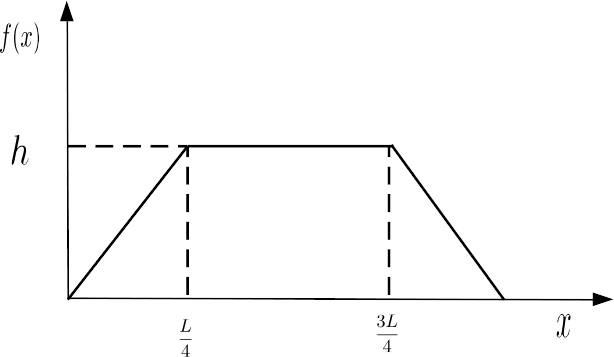
\includegraphics{review2_fig.png}
\end{figure}
Using MATLAB syntax, complete the local function shown in the space below:
\begin{lstlisting}[style=myMatlab, frame=none, numbers=none]
%% Local Function to implement IC
function y = ICfun(x)
[m,n] = size(x);
y = nan(m,n);

for i = 1:length(x)










end
end
\end{lstlisting}

\end{enumerate}

\end{fullwidth}
